%% =====================================================================
%%  University Physics Competition (UPC) -- official-style paper template
%%  Based on 2010-2025 Gold Medal papers (see references/layout-conventions.md)
%%
%%  Compile:  bash scripts/build.sh paper.tex
%%  Check  :  python3 scripts/check_pdf.py paper.pdf
%%
%%  HARD RULES enforced by this template
%%   - page 1 holds ONLY: team number, problem letter, title, summary (<=300 words)
%%   - team number appears in the header of EVERY page
%%   - no student names / institution anywhere
%% =====================================================================
\documentclass[12pt,letterpaper]{article}

% ---------- page geometry & typography -------------------------------
\usepackage[letterpaper,margin=1in,headheight=14pt,headsep=18pt]{geometry}
\usepackage[T1]{fontenc}
\usepackage[utf8]{inputenc}
\usepackage{lmodern}
\usepackage{microtype}
\usepackage{setspace}
\setstretch{1.08}

% ---------- math ------------------------------------------------------
\usepackage{amsmath,amssymb,amsfonts,bm}
\usepackage{siunitx}
\sisetup{detect-all,per-mode=symbol,exponent-product=\times}

% Superscripts default to 8 pt against 12 pt body (67 %), which makes unit
% exponents such as s^{-1} look heavy; 64 % is easier next to the letters.
\DeclareMathSizes{12}{12}{7.8}{5.6}
% Compact negative exponent for units: \inv gives ^{-1} with the spaces on
% both sides of the minus removed, so "m s\inv" sets as m s^-1 instead of
% the loose "m s - 1" that a plain ^{-1} produces at script size.
% Compact negative exponent for units: the math minus keeps its full
% advance at script size, so a plain ^{-1} sets as a long dash floating away
% from the digit.  \inv scales the minus horizontally to 65 %, keeps it on the
% script axis and closes the spacing, so "m s\inv" reads as m s^-1 while the
% PDF still contains a real minus character.
\newcommand{\inv}{\textsuperscript{\scalebox{0.65}[1]{$-$}1}}

% ---------- floats, tables, figures ----------------------------------
\usepackage{graphicx}
\usepackage{booktabs}
\usepackage{multirow}
\usepackage{array}
\usepackage{float}
\usepackage[font=small,labelfont=bf,justification=centering]{caption}
\usepackage{subcaption}
\usepackage[section]{placeins}

% ---------- lists, code, links ---------------------------------------
\usepackage{enumitem}
\setlist{itemsep=2pt,topsep=3pt,parsep=0pt}
\usepackage{listings}
\lstdefinestyle{aiquote}{basicstyle=\ttfamily\footnotesize,breaklines=true,
        frame=leftline,framerule=0.4pt,columns=fullflexible,
        showstringspaces=false,xleftmargin=1.2em,framesep=4pt,
        aboveskip=0.4em,belowskip=0.8em}
\lstset{basicstyle=\ttfamily\footnotesize,breaklines=true,frame=single,
        numbers=left,numberstyle=\tiny,columns=fullflexible}
\usepackage{xcolor}
\usepackage{tocloft}
\setcounter{tocdepth}{2}
\renewcommand{\contentsname}{Contents}
\renewcommand{\cfttoctitlefont}{\large\bfseries}
\renewcommand{\cftaftertoctitle}{\par\vspace{0.4em}\hrule\vspace{0.8em}}
\renewcommand{\cftsecfont}{\bfseries}
\renewcommand{\cftsecpagefont}{\bfseries}
\setlength{\cftbeforetoctitleskip}{0pt}
\renewcommand{\cftsecleader}{\cftdotfill{\cftdotsep}}
\renewcommand{\cftsubsecleader}{\cftdotfill{\cftdotsep}}
\renewcommand{\cftdotsep}{1.2}
\usepackage[colorlinks=true,linkcolor=black,citecolor=black,
            urlcolor=blue!45!black]{hyperref}

% ---------- running head: TEAM NUMBER ON EVERY PAGE ------------------
\usepackage{fancyhdr}
\pagestyle{fancy}
\fancyhf{}
\fancyhead[L]{\small Team \teamnum}
\fancyhead[R]{\small Problem \problemltr}
\fancyfoot[C]{\small\thepage}
\renewcommand{\headrulewidth}{0.4pt}
\fancypagestyle{plain}{\fancyhf{}\fancyhead[L]{\small Team \teamnum}%
  \fancyhead[R]{\small Problem \problemltr}\fancyfoot[C]{\small\thepage}%
  \renewcommand{\headrulewidth}{0.4pt}}

% ---------- fill these in ---------------------------------------------
\newcommand{\teamnum}{000}          % <-- your team number
\newcommand{\problemltr}{A}         % <-- A or B
\newcommand{\papertitle}{Full Paper Title Written in Title Case}

% Set \aiusedtrue if a generative AI tool influenced text, code, figures or
% analysis; the "Report on the Use of AI" then appears at the end.
\newif\ifaiused
\aiusedfalse

% ---------- macros (keep consistent notation across the team) --------
\newcommand{\dd}{\mathrm{d}}
\newcommand{\ee}{\mathrm{e}}
\newcommand{\ii}{\mathrm{i}}
\newcommand{\vect}[1]{\bm{#1}}
% siunitx v3 already provides \qty and \unit; use those directly.

\begin{document}

% =====================================================================
% PAGE 1 -- exactly four items. Nothing else. No names, no school.
% =====================================================================
\begin{titlepage}
\thispagestyle{empty}
\vspace*{0.6cm}
\noindent
\begin{minipage}[t]{0.45\textwidth}
  {\scshape Problem}\\[0.35em]{\LARGE\bfseries \problemltr}
\end{minipage}%
\hfill
\begin{minipage}[t]{0.45\textwidth}
  \raggedleft
  {\scshape Team}\\[0.35em]{\LARGE\bfseries \teamnum}
\end{minipage}

\vspace{1.1em}
\noindent\rule{\linewidth}{0.5pt}
\vspace{1.7em}

\begin{center}
  {\LARGE\bfseries \papertitle}
\end{center}

\vspace{1.7em}
\begin{center}
  % "Abstract" is equally accepted; 64 of the 74 gold papers use that word.
  {\large\scshape Summary}
\end{center}

\begingroup
\setstretch{1.06}
\setlength{\leftskip}{0.05\textwidth}
\setlength{\rightskip}{0.05\textwidth}
\noindent
% ---- <=300 words. Must contain: what was done, assumptions, answers to
% ---- every question asked, final numbers, conclusions. scripts/check_pdf.py
% ---- counts the words for you.
State the physical situation in one sentence. Then say what model you built
and which assumptions carry it (e.g.\ rigid body, steady state, neglect
radiation pressure). Then answer each question of the problem in order, with
the numbers and their units, e.g.\ ``the time to reach the threshold is
\SI{38}{s} for the nominal case''. Close with one sentence on validation
(comparison with published data or a limiting case) and one on the main
uncertainty.
\par
\endgroup

\vfill
\end{titlepage}
\setcounter{page}{2}% titlepage resets the counter; restore continuous numbering

% ---------- contents ---------------------------------------------------
% 50 of the 74 gold papers print a Contents page; drop it if you prefer not.
\tableofcontents
\clearpage

% =====================================================================
% BODY
% =====================================================================
\section{Introduction}
\label{sec:intro}
Background in 2--3 paragraphs: why the scenario matters, what is already
known, what makes it hard. End with a short roadmap of the paper.
Cite sources as you go, e.g.\ the classical blow-down analysis of
Ref.~\cite{shapiro1953,anderson2003}.
State the contribution explicitly: ``In this paper we derive \ldots, validate
it against \ldots, and obtain \ldots.''

\section{Problem Restatement and Clarification}
\label{sec:problem}
Restate the problem in your own words. Define the quantities that are asked
for and their symbols. If the statement is ambiguous, say which
interpretation you adopt and why.

\section{Assumptions and Notations}
\label{sec:assumptions}
Every assumption gets a reason and, where possible, a quantitative check that
it is harmless (order-of-magnitude estimate). Tables read well here.

\begin{table}[htbp]
  \centering
  \caption{Assumptions and the justification for each.}
  \label{tab:assumptions}
  \begin{tabular}{@{}lll@{}}
    \toprule
    \# & Assumption & Justification / validity check \\
    \midrule
    A1 & Air is an ideal gas & Knudsen number $\ll 1$ for $p>\SI{0.01}{atm}$ \\
    A2 & Quasi-steady outflow & hole diameter $\ll$ station length \\
    A3 & Isothermal walls & 48\,h time scale $\gg$ thermal relaxation \\
    \bottomrule
  \end{tabular}
\end{table}

\section{Physical Model}
\label{sec:model}
Build the model in layers. For each layer state the governing equation and
its regime of validity. Number every equation you refer to later.

\begin{equation}
  \frac{\dd p}{\dd t} = -\frac{\gamma p A}{V}\,u(p), \qquad
  u(p) = \sqrt{\frac{2\gamma}{\gamma-1}\frac{p}{\rho}\left[1-\left(\frac{p_a}{p}\right)^{(\gamma-1)/\gamma}\right]}
  \label{eq:blowdown}
\end{equation}

Explain each symbol right after it appears, then check dimensions
($[\mathrm{Pa/s}]$ on both sides).

\section{Method and Numerical Solution}
\label{sec:method}
Describe the algorithm, parameters, step size, convergence criterion and
runtime. State what software was used and cite it. Reproducibility matters
more than sophistication.

\section{Results}
\label{sec:results}
One subsection per question asked in the problem statement. Each subsection:
state the answer, give the number with units and uncertainty, show the figure
that supports it, and one sentence interpreting it.

\begin{figure}[htbp]
  \centering
  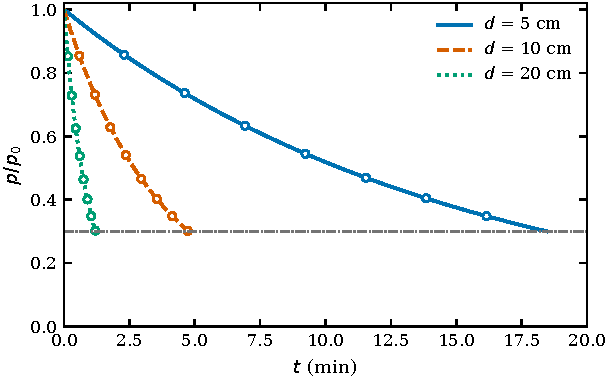
\includegraphics[width=0.72\textwidth]{figures/example.pdf}
  \caption{Pressure ratio $p/p_0$ versus time for three hole diameters
  (solid, dashed, dotted). Replace with your own figure: vector PDF,
  axes labelled with the physical quantity and its unit, one caption
  sentence stating what is plotted and what the reader should see.}
  \label{fig:blowdown}
\end{figure}

\begin{table}[htbp]
  \centering
  \small
  \caption{Time to reach $0.3\,p_0$ versus hole diameter.}
  \label{tab:results}
  \begin{tabular}{@{}S[table-format=2.0]S[table-format=4.1]@{}}
    \toprule
    {$d$ (cm)} & {$t$ (s)} \\
    \midrule
     5 & 1108.0 \\
    10 &  285.5 \\
    20 &   72.5 \\
    \bottomrule
  \end{tabular}
\end{table}

\section{Discussion}
\label{sec:discussion}
Compare with independent data or a limiting case (see \cite{shapiro1953,landau1987}). Quantify sensitivity to the
weakest assumption ($\pm20\%$ in $C_d$ changes $t$ by \ldots). List the error
sources and their size. Say what would change your conclusion.

\section{Strengths and Weaknesses}
\label{sec:sw}
\textbf{Strengths.}
\begin{enumerate}[label=(\arabic*)]
  \item The model reproduces the published blow-down curve within 8\%.
  \item Assumptions are checked, not merely stated.
  \item Results are given as closed-form scaling laws usable outside the
        specific numbers of the problem.
\end{enumerate}
\textbf{Weaknesses.}
\begin{enumerate}[label=(\arabic*)]
  \item Choked flow is assumed throughout; near $0.3\,p_0$ this overestimates
        the mass flux by \ldots\%.
  \item Wall friction and heat transfer are neglected.
\end{enumerate}

\section{Conclusion}
\label{sec:conclusion}
Answer each question of the problem in one numbered sentence, with the final
numbers repeated. Then one sentence on the broader takeaway.

% =====================================================================
\section*{References}
\addcontentsline{toc}{section}{References}
\begin{thebibliography}{9}
% Real entries, so the skeleton compiles with a plausible reference list.
% Replace them with the sources your paper actually used and verify each one.
\bibitem{shapiro1953} A.~H. Shapiro, \emph{The Dynamics and Thermodynamics of
Compressible Fluid Flow}, vol.~1 (Ronald Press, New York, 1953).
\bibitem{anderson2003} J.~D. Anderson, \emph{Modern Compressible Flow: With
Historical Perspective}, 3rd ed.\ (McGraw-Hill, New York, 2003).
\bibitem{landau1987} L.~D. Landau and E.~M. Lifshitz, \emph{Fluid Mechanics},
vol.~6 of Course of Theoretical Physics, 2nd ed.\ (Pergamon, Oxford, 1987).
\bibitem{press2007} W.~H. Press, S.~A. Teukolsky, W.~T. Vetterling and
B.~P. Flannery, \emph{Numerical Recipes: The Art of Scientific Computing},
3rd ed.\ (Cambridge University Press, Cambridge, 2007).
\end{thebibliography}

\appendix
\section{Derivation of Eq.~\eqref{eq:blowdown}}
\label{app:derivation}
Long algebra goes here; the main text must already explain the method.

\section{Code}
\label{app:code}
\begin{lstlisting}[language=Python,caption={Integration of Eq.~\eqref{eq:blowdown}.}]
import numpy as np
def blowdown(p0=101325.0, V=628.0, A=7.85e-5, gamma=1.4, dt=1e-3):
    ...
\end{lstlisting}

% ---- required only if generative AI was used (official rule 5) ------
% The full version of this section, with a systems table, a query table and
% one block per output, lives in templates/project/sections/11-ai-report.tex.
\ifaiused
\section*{Report on the Use of AI}
\addcontentsline{toc}{section}{Report on the Use of AI}

\noindent\textbf{Systems:} \verb|GPT-5| (OpenAI, 2025-10), web chat.

\subsection*{Work carried out without AI}
State here what the team did itself; see the project template for the
wording used in gold papers.

\subsection*{Queries (verbatim)}
\paragraph{Query 1.}
\begin{lstlisting}[style=aiquote]
<paste the exact text typed into the tool>
\end{lstlisting}

\subsection*{Outputs (complete)}
\paragraph{Output 1.}
\begin{lstlisting}[style=aiquote]
<paste the complete output>
\end{lstlisting}
\fi

\end{document}
